\chapter{shadowLB}
\label{proposal}

本章では,\ref{issue}章にて述べた問題点を解決するための基盤,shadowLBを実現手法の設計に関して論じる


\section{概要}



% \section{BGP}
% \subsection{概要}
% BGPとはインターネットにおいて自律システム\footnote{Autonomous System. インターネットを構成するネットワークをそれぞれ独立的に運用する組織群を指す.}間の経路情報交換に用いられるパスベクタ型の動的経路制御プロトコルである.現在有効なバージョンはBGP4であり,RFC4271で定義されている\cite{RFC4271}.


% \subsection{用語}
% BGPにおいて利用される用語のうち,本提案手法において重要なものを以下に列記する.

% \subsubsection{BGPスピーカ}
% BGPを実装された機器をBGPスピーカと呼ぶ.

% \subsubsection{BGPピア}
% BGPで経路交換を行う関係にある機器をぞれぞれBGPピア(BGP Peer)と呼称する.

% そのうち,自律システム間での接続関係にあるピアをEBGP(External BGP)ピア,同一自律システム内のBGPスピーカ同士の経路交換に用いられるピアをIBGP(Internal BGP)ピアと呼ぶ.

% \subsubsection{BGPコネクション}
% BGPコネクションとはBGPで経路交換に用いられる接続関係を指す.各機器は1対1の関係でBGPコネクションを確立する.
% BGPコネクションにはトランスポート層のプロトコルとして{TCP\cite{RFC793}のポート番号179が利用され,フラグメンテーションや再送制御,応答確認,誤り制御等,TCPによる高信頼なメッセージングが可能である.

% また,BGPコネクションを維持・管理するために,BGPでは以下のような4つのメッセージが定義されている.

% BGPコネクションはBGPピア間でTCPコネクションを確立したのちにOPENメッセージにより各機能の対応関係を確認することにより確立され,KEEPALIVEメッセージによりセッションが維持される.UPDATEメッセージにより,BGPピアへ広告する経路(Adj-RIB-Out)に変更が生じたことを通知する.何らかの理由によりBGPコネクションが確立出来なくった場合,NOTIFICATIONメッセージを利用して切断を通知する.

% \subsubsection{Adj-RIB-In/Adj-RIB-Out/Loc-RIB}
% \begin{figure}[h]
%     \begin{center}
%     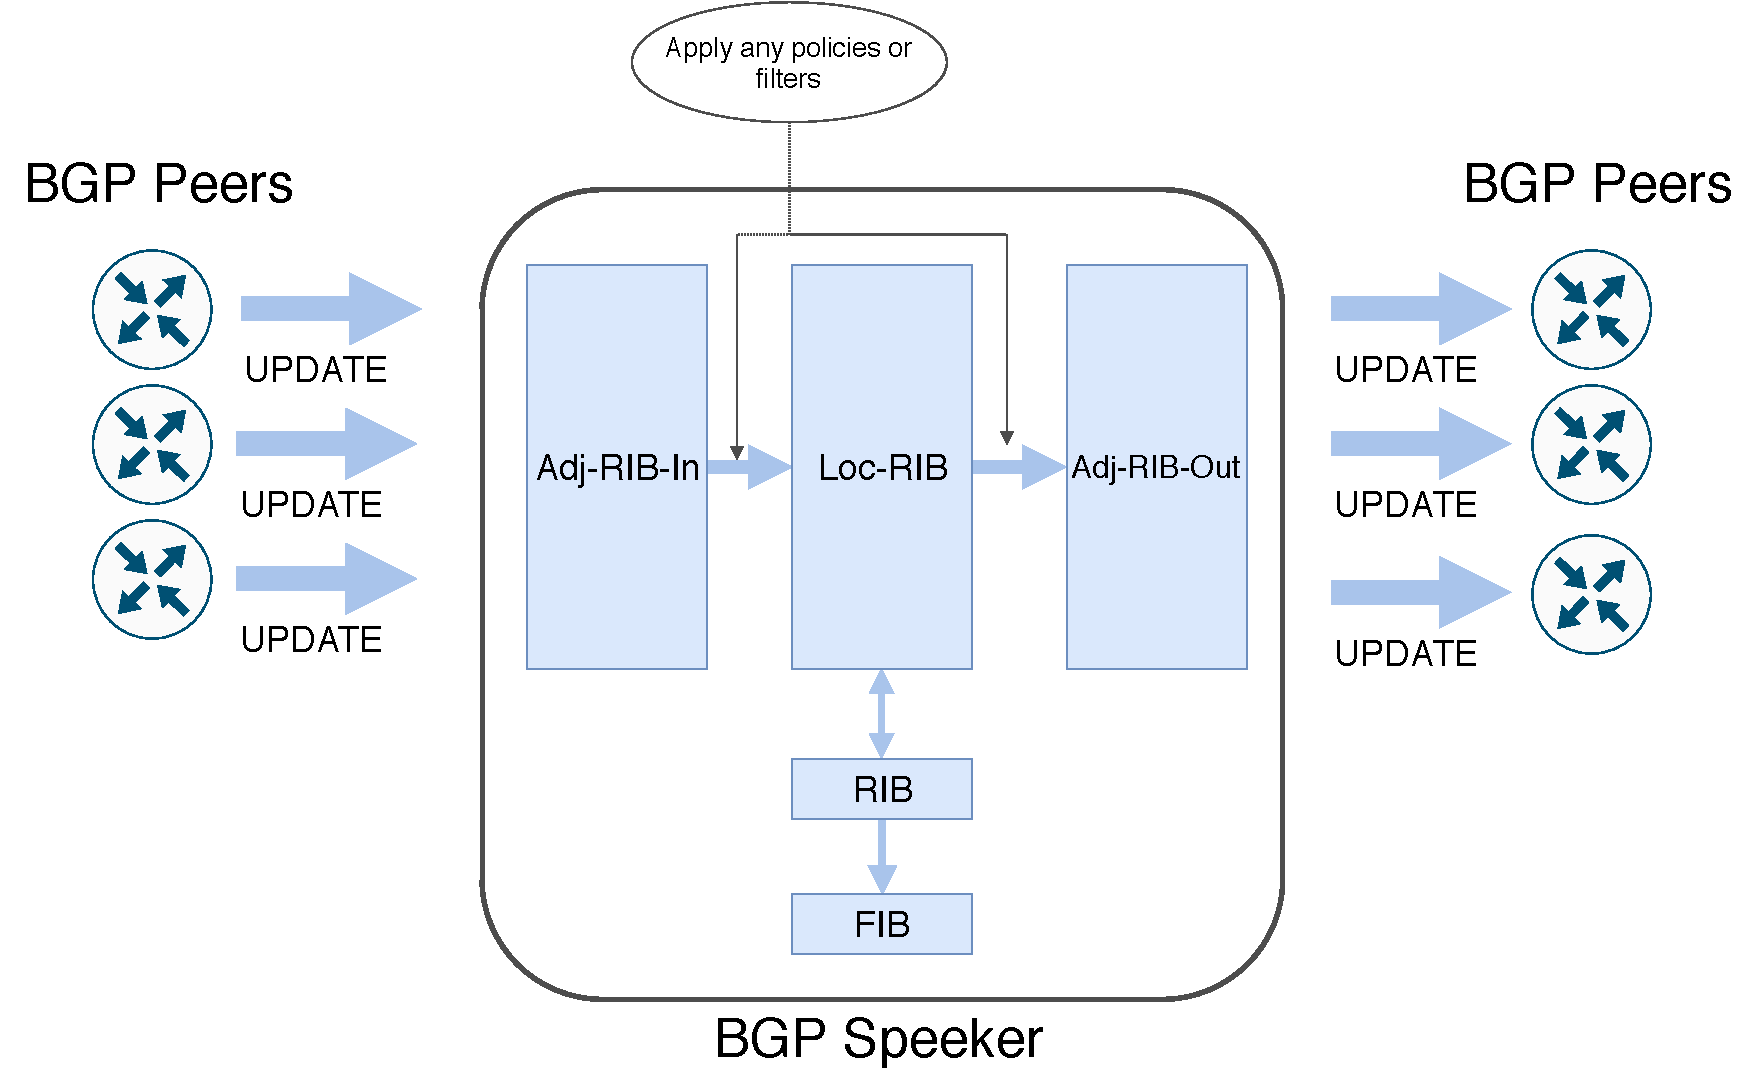
\includegraphics[width=10cm,pagebox=cropbox,clip]{img/bgp-rib-model.pdf}
%     \end{center}
%     \caption{BGPスピーカの経路の扱い}
%     \label{fig:bgp-rib-model}
% \end{figure}
% 図\ref{fig:bgp-rib-model}にBGPにおける経路受信・保持・送信の流れを示す.
% BGPピアから受信した経路はAdj-RIB-Inと呼ばれ,BGPスピーカの任意のフィルターやポリシーを適用した上でLoc-RIBと呼ばれるテーブルに保存される.
% BGPスピーカはLoc-RIBから任意のフィルターを適用した経路をBGPピアに広告する.この広告する経路をAdj-RIB-Outと呼ぶ.




% \subsection{特徴}
% 本提案手法においてダイナミックEAMTを実現するためのメッセージングプロトコルとしてBGPを選択するに至った要素について述べる.

% \subsubsection{マルチプロトコル}
% 現行版であるBGP4では,OPENメッセージにオプション値(Capabilities Optional Parameter)を挿入することで,IANAによって定められた任意のネットワークプロトコル\cite{IANA_AFI,IANA_SAFI}の経路を交換することが想定されている\cite{RFC4760}.本提案手法で利用しているIPv6ユニキャスト経路もこの機構を用いる.


% \subsubsection{実装が一般的}
% BGPは自律システム間の経路交換プロトコルとしてインターネットで利用されているデフファクトスタンダードなプロトコルであり,OSS(Open Source Software)\footnote{ソースコードが公開されており,定められたライセンス規約に基づく範囲で自由に使用・改造が可能なソフトウェア.}にも多くの実装が存在する.
% 広く普及したプロトコルを利用することにより,特別な実装を最小限にして本提案手法を実現することが出来る.

% \subsubsection{中継ネットワークに非依存}
% 本提案手法で採用しているIBGPでは,TTL(Time to Live)\footnote{そのパケットが宛先ホストに到達するまでに許容される中継ルータ数.IPv6プロトコルではHop Limitとして同一の機能が実装されている\cite{RFC8200}.}が255に設定されており,BGPピア間でIPv4/IPv6による到達性があればメッセージングを行うことが可能である.すなわち本提案手法は既存のSIIT-DCネットワークに非依存であり,これは第\ref{consideration:points}項で述べた要件の一つである,デプロイメントの容易さを充足する.


% \section{基本的なネットワーク設計}
% \label{proposal:network}
% \begin{figure}[h]
%     \begin{center}
%     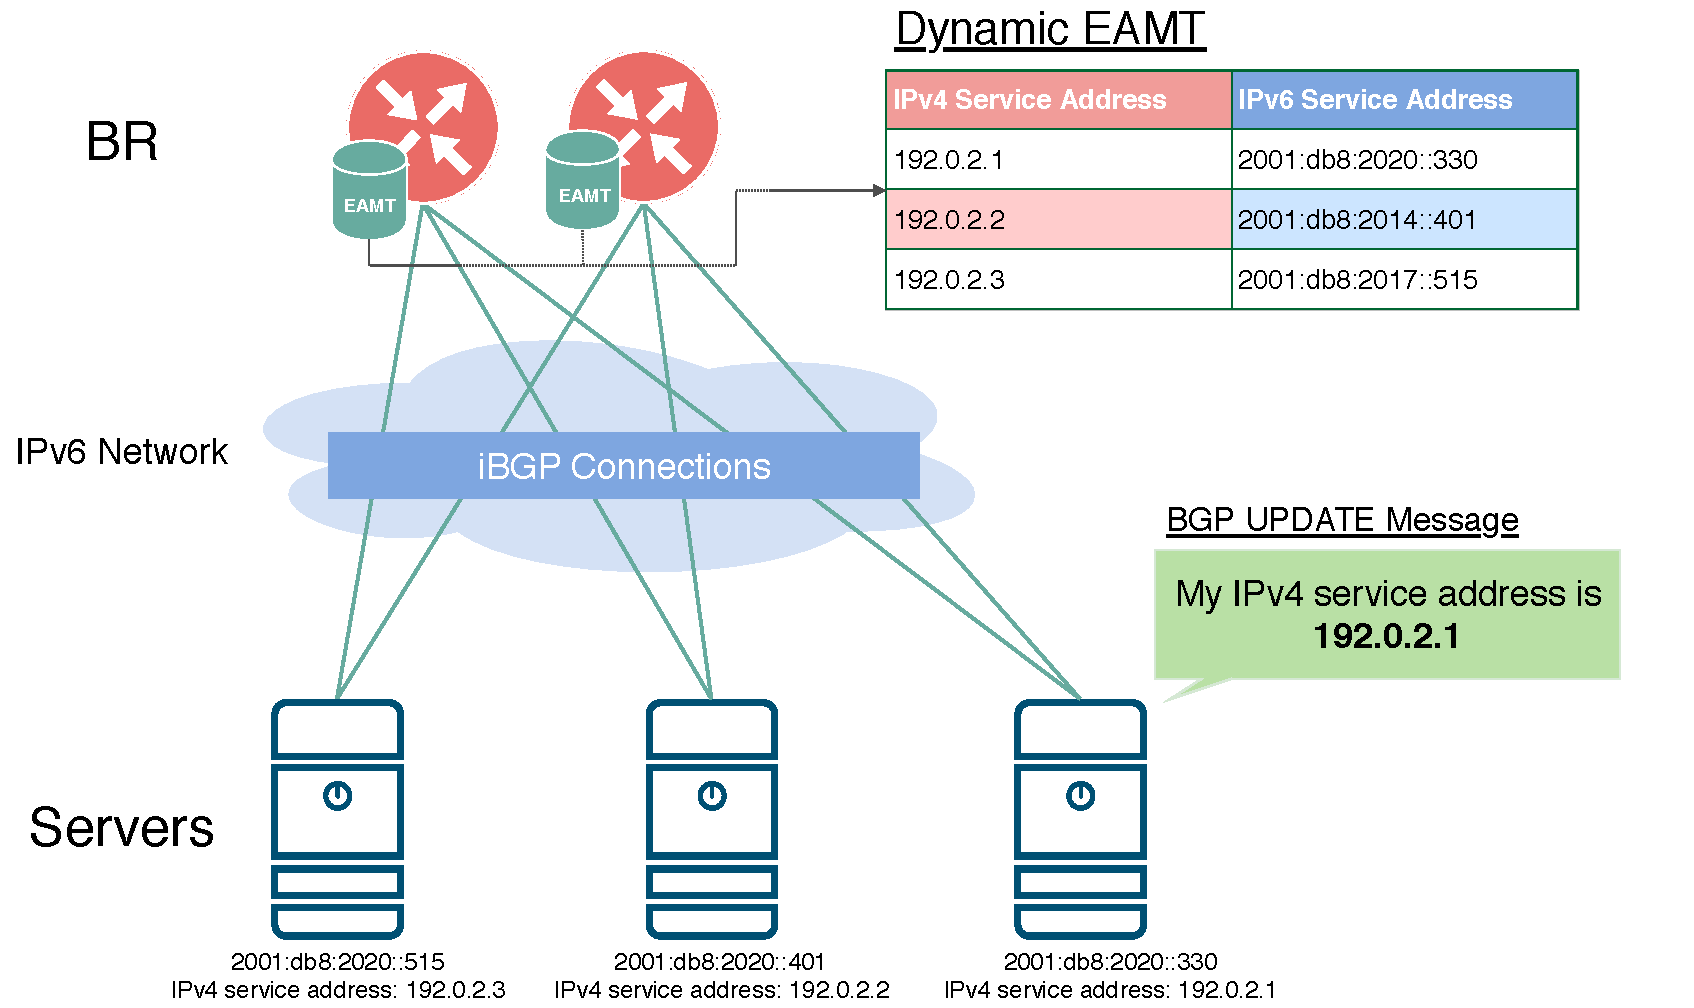
\includegraphics[width=15cm,pagebox=cropbox,clip]{img/proposal_method_network.pdf}
%     \end{center}
%     \caption{本提案手法の基本機能を実装したSIIT-DCネットワークの例}
%     \label{fig:proposal_method_network}
% \end{figure}


% 図\ref{fig:proposal_method_network}本提案手法の各要素の関係を示す.

% BR数を$N$,サーバ数を$M$とした,ルートリフレクタを利用した本提案手法での必要なBGPコネクション数$C_a$は式\ref{eq:proposal_network}のように表現できる.

% \begin{equation}
%     \label{eq:proposal_network}
%     C_a = M \cdot N
% \end{equation}


% \subsection{各ノードの役割と機能要件}
% \label{proposal:network:nodes}
% \subsubsection{BR}
% BRでは下記のような3つの機能が必要となる.
% \begin{itemize}
%     \item BGPデーモン\\
%     各サーバとIBGPコネクションを確立し,Loc-RIBを生成する.
%     \item SIIT機構\\
%     EAMTを保持し,それを参照してIPv4/IPv6プロトコル変換を行う.
%     \item EAMT制御機構\\
%     BGPデーモンが有するのLoc-RIBを参照し,EAMTを更新する.
% \end{itemize}

% \subsubsection{IPv4サービス提供サーバ}
% IPv4サービス提供サーバでは以下の2つの機構が求められる.
% \begin{itemize}
%     \item IPv4サービス\\
%     IPv4によりインターネットに提供したいサービスを稼働させる.
%     \item BGPデーモン\\
%     自身が提供するIPv4サービスアドレスを含んだ情報を広告する.
% \end{itemize}


% \section{ルートリフレクタを活用したネットワーク設計}
% \label{proposal:network_rr}
% \begin{figure}[h]
%     \begin{center}
%     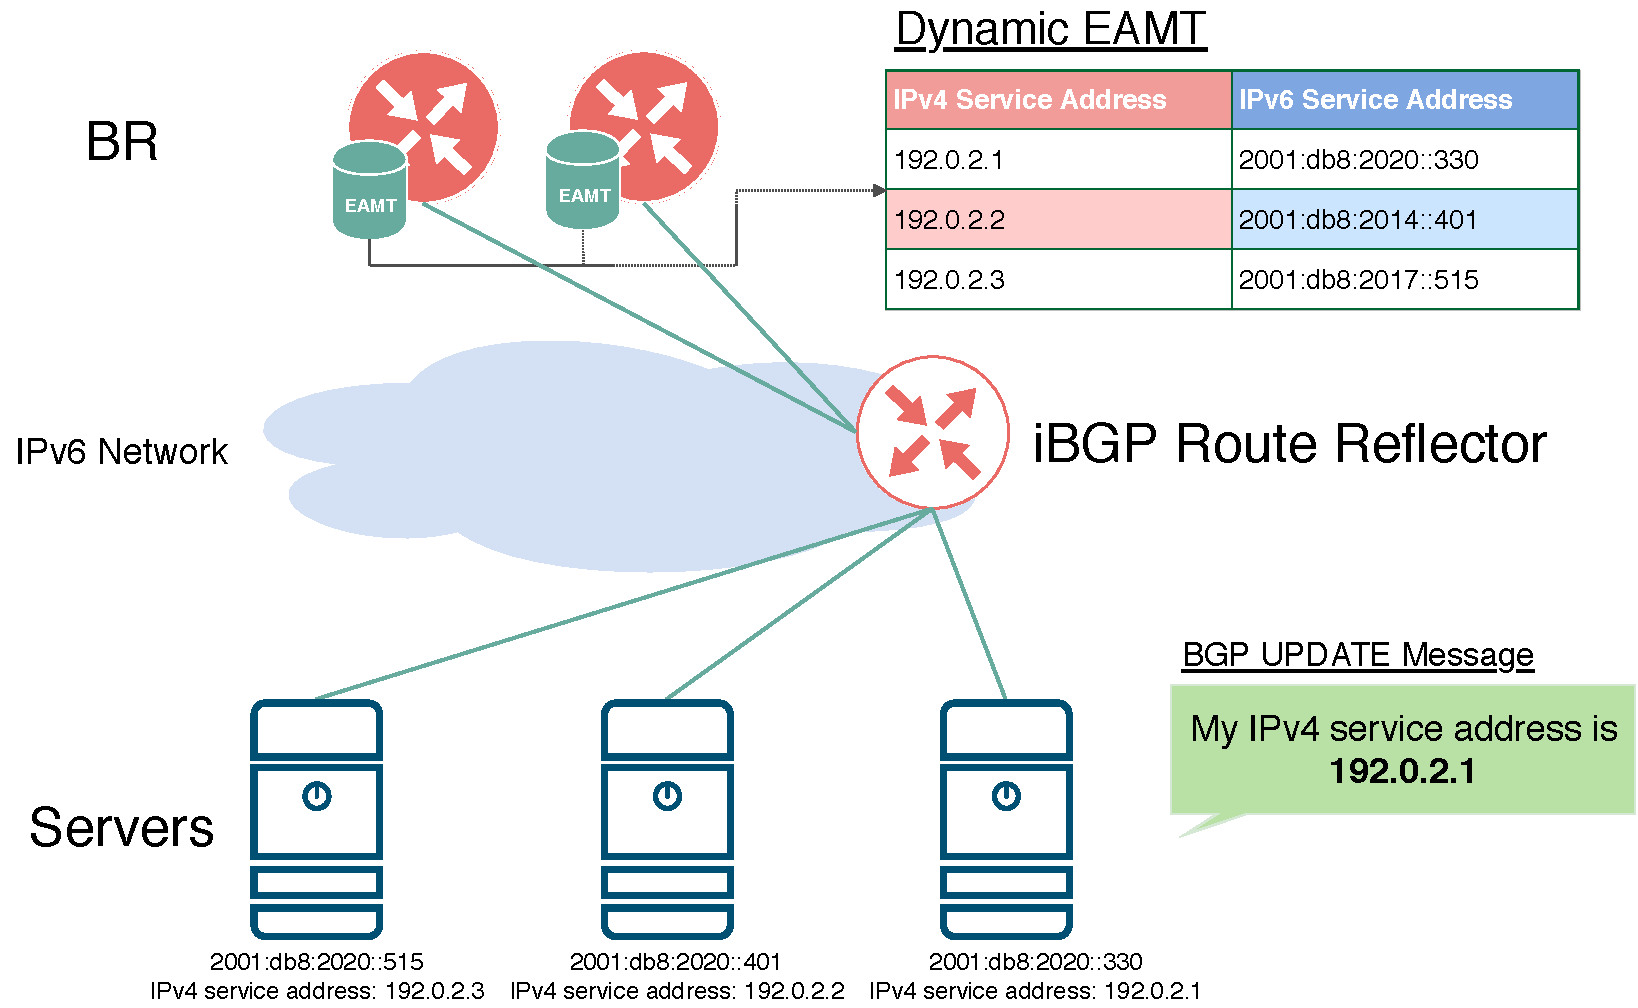
\includegraphics[width=15cm,pagebox=cropbox,clip]{img/proposal_method_network_rr.pdf}
%     \end{center}
%     \caption{ルートリフレクタを採用したSIIT-DCネットワークの例}
%     \label{fig:proposal_method_network_rr}
% \end{figure}

% 通常,IBGPではルートループを防ぐために異なるBGPピアから受信した経路は他のBGPピアに広告されない.そのため一つのIBGPスピーカが広告する経路を他のIBGPスピーカが受信するためには,BGPコネクションをフルメッシュで確立する必要がある\cite{vutukuru2005construct}.

% ルートリフレクタとは,Originator-IDと呼ばれる特殊な属性をAdj-RIB-Outに付与することでルートループを防ぎながら,IBGPピアから受信した経路を他のIBGPに対して広告する特殊なBGPスピーカである\cite{RFC4456}.ルートリフレクタはIBGPのコネクション数を削減するために広く利用されている.

% ルートリフレクタを複数設置することで,負荷分散・冗長化構成を容易に実現することが出来る.一般的にはルートリフレクタ間はフルメッシュでのBGPコネクションを確立する設計を行うが,
% Gutiérrezらによればツリー型のBGPコネクション関係を一部で選択することにより,よりルートリフレクタに掛かる負荷を軽減出来ることが明らかになっている\cite{6838346}.

% BR数を$N$,サーバ数を$M$,ルートリフレクタの数を$L$とした,ルートリフレクタを利用した本提案手法での必要なBGPコネクション数$C_b$は式\ref{eq:proposal_network_rr}のように表現できる.なおルートリフレクタ間のBGPコネクションはフルメッシュを想定している.
% 第\ref{proposal:network}節で述べた基本的なネットワーク設計を行う場合と比較して,SIIT-DCネットワークが大きくなった場合にBGPコネクションが大幅に削減できることがわかる.


% \begin{equation}
%     C_b = \frac{L(2M + 2N + L - 1)}{2}
%     \label{eq:proposal_network_rr}
% \end{equation}

% \subsection{各ノードの役割と機能要件}
% \subsubsection{BR及びIPv4提供サーバ}
% BR及びIPv4サービス提供サーバは,ルートリフレクタとのみBGPコネクションを確立する.複数ルートリフレクタを配備する場合,それぞれとコネクションを確立することで冗長性を高めることが出来る.
% その他の機能は第\ref{proposal:network}で述べたものと同様に配備する.

% \subsubsection{ルートリフレクタ}
% ルートリフレクタでは,ルートリフレクタ機能が有効となったBGPデーモンを配備する必要がある.各サーバ・BRとBGPコネクションを確立する.


% \section{各アプローチとの比較}
% \label{proposal:compare}
% 第\ref{consideration:approach}節で検討した各アプローチと本提案手法を,第\label{consideration:points}節で挙げた各性能要件に関して比較する.


% \begin{table}[h]
%     \caption{各手法の比較}
%     \label{table:compare_proposal}
%     \resizebox{\textwidth}{!}{%
%     \begin{tabular}{lcccc}
%     \hline
%     手法                                                                & EAMTの一貫性 & 変更追従性                                                   & コネクション数 & デプロイメントの容易さ                                                  \\ \hline
%     参考:\\ オペレーターによる手動設定                                                & 無し               & 無し                                                       & ------            & -----                                                        \\ \hline
%     中央管理型アプローチ                                                        & 有り               & \begin{tabular}[c]{@{}c@{}}\\ (監視機構の実装依存)\end{tabular} & $\frac{L(2M + 2N + L - 1)}{2}$         & \begin{tabular}[c]{@{}c@{}}\\ 困難(コントローラーの実装依存)\end{tabular}   \\ \hline
%     分散管理型アプローチ                                                        & 無し               & 有り                                                       & $M \cdot N$        & 有り                                                            \\ \hline
%     \begin{tabular}[c]{@{}l@{}}提案手法1:\\ IBGP\end{tabular}             & 有り               & 有り                                                       & $M \cdot N$               & 容易                                                            \\ \hline
%     \begin{tabular}[c]{@{}l@{}}提案手法2:\\ IBGP + ルートリフレクタ\end{tabular} & 有り               & 有り                                                       & $\frac{L(2M + 2N + L - 1)}{2}$                  & \begin{tabular}[c]{@{}c@{}}容易\\ (RRは容易にスケールアウト可能)\end{tabular} \\ \hline
%     \end{tabular}%
% }
% \end{table}
% 表\ref{table:compare_proposal}にそれぞれの項目における比較結果を示す.なお,コントローラーもしくはルートリフレクタの導入数を$L$,サーバ数を$M$,BRの数を$N$としている.

% \subsection{EAMTの一貫性}
% BGPはインターネットの経路広告手法として広く利用されており,多数のルータ間で一定の一貫性を保つことがプロトコルレベルで保証されている.
% 本提案手法ではBGPを利用したメッセージングにより,SIIT-DCネットワークにおけるダイナミックEAMTを実現しているため,BGPと同水準の一貫性の担保が可能である.


% \subsection{変更追従性}
% 本提案手法では各IPv4サービス提供サーバが自身のEAMをBGPの経路情報として広告するため,サーバが広告するモデルを採用する分散管理型アプローチと同様に,経路広告の有無によりサーバのネットワーク健全性を保証する事ができる.

% 一方で\ref{consideration:approach:centerized}項で述べたように,中央管理型アプローチにおいても変更追従性を実現可能であるが,コントローラの監視機構の実装に依存するほか,何らかの手段によってマスターテーブルに対して変更を適用する手段を考慮する必要がある.


% \subsection{コネクション数}
% 各サーバが直接BRに対してコネクションを確立する分散管理型アプローチ及び提案手法1では,サーバ・BRの数が大きくなった場合に,EAMTの維持・管理に必要なコネクション数が増加する.

% 一方でルートリフレクタを採用した提案手法2と中央管理型アプローチでは,サーバ・BRの数が増加した場合にも,上記2手法と比較して少ないコネクションでEAMTを維持・管理することが可能である.


% \subsection{デプロイメントの容易さ}
% 本提案手法では動的経路制御プロトコルとして一般的なBGPをメッセージングに利用しているため,OSSを含む多種多様な実装をそのまま利用することが可能であり,他の手法と比較して実装・デプロイメントが容易である.

% また\ref{proposal:network_rr}節で述べたように,ルートリフレクタ間のトポロジや管理方法を工夫することで,更なるコネクション数とルートリフレクタの負荷軽減を実現する余地がある.

% 一方で,中央管理型アプローチでは,特別な監視・管理機構を持ったコントローラを実装する必要があり,他のデプロイメントの障壁が高くなる.




%%% Local Variables:
%%% mode: japanese-latex
%%% TeX-master: "../bthesis"
%%% End:
